\section{Introduction}
\label{sec:intro}

% Replacement for figures/motivation.tex in the v14 Overleaf project.
% Requires tikz, xcolor, graphicx and arrows.meta (already loaded by main.tex).
\begin{figure*}[t]
\centering
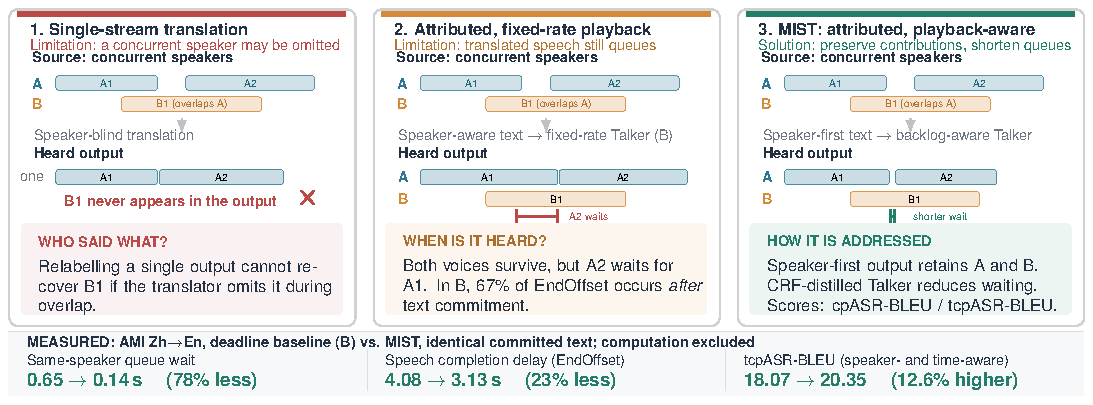
\includegraphics[height=5cm]{figures/MIST_Figure1_Motivation_Redesigned.pdf}
\caption{Motivation. (1)~Speaker-blind single-stream translation may omit overlapping contributions. (2)~Speaker attribution alone leaves playback queues: 67\% of the deadline baseline's EndOffset occurs after text commitment (queue plus final-block playback; Table~\ref{tab:decomp}). (3)~\sys{} combines speaker-first decoding with a backlog-aware Talker trained on the posterior of a playback-queue CRF; no CRF runs online. Bottom: measured improvements on AMI Zh$\rightarrow$En over the baseline with identical text, excluding computation. All utterance timelines are schematic.}
\label{fig:motivation}

\end{figure*}





Simultaneous speech-to-speech translation (SimulS2ST) is increasingly explored for real-time multilingual communication, such as online meetings, where speech serves as the primary medium for understanding and interaction across languages \citep{seamless2023,labiausse2025hibiki,cheng2025liveinterpret}.
In these real-world conversations, frequent speaker changes and overlapping utterances complicate the input audio, turning distinct contributions into a multi-talker stream whose content must be attributed to the correct speaker \citep{carletta2005ami,yang2024diarist}.
This multi-talker speech is then translated and synthesised into speaker-specific output streams, where each generated segment can queue behind earlier speech from the same speaker and delay what listeners actually hear. While quantifying these effects in streaming SimulS2ST remains challenging, existing studies typically rely on text translation quality and text-emission latency \citep{ma2019stacl,papi2022over}, proxies that do not jointly capture speaker-attributed speech quality and listener-side playback delay.

To provide low-latency translation, many simultaneous speech-to-speech translation (SimulS2ST) systems process one active speaker at a time and focus on when translated content is emitted \citep{seamless2023,labiausse2025hibiki,cheng2025liveinterpret,deng2025simuls2s}.
In multi-talker meetings, however, overlapping speech challenges this assumption, as speaker-blind translation can omit concurrent contributions that subsequent speaker attribution cannot recover.
Although speaker tracking and voice cloning can associate generated speech with speaker identities \citep{zhao2026xtranslator}, they do not account for the playback queues that delay later translations from the same speaker.
Moreover, text-level translation metrics and text-emission latency do not directly capture speaker-attributed speech quality or when translated words are actually heard; in our baseline, approximately two-thirds of utterance completion delay occurs after text commitment (Figure~\ref{fig:motivation}).
These limitations motivate a simultaneous S2ST framework that preserves concurrent contributions, models speaker-specific playback queues, and evaluates the translated speech heard by listeners.

We introduce \sys{} (\emph{Meeting Interpretation with Speaker Tracking}), a SimulS2ST framework that produces separate, speaker-attributed spoken translations in multi-talker meetings, including overlapping speech. By interleaving acoustic tokens with speaker tokens from a frozen streaming diarizer, \sys{} generates speaker-first, time-stamped translations, which a voice-prompted Talker renders in each speaker's voice. For listener-side delay, we introduce backlog-dependent speaking rates and \emph{playback alignment} (PA), a linear-chain CRF that balances rendering quality against the delay each candidate imposes on both current and subsequent speech. By training the Talker on its latency-constrained posterior, PA makes speech generation aware of future playback costs without requiring CRF inference at test time. We further introduce novel cpASR-BLEU and tcpASR-BLEU to evaluate synthesised speech with speaker attribution and, for the latter, temporal constraints. Across whole AMI and AliMeeting meetings, \sys{} improves tcpASR-BLEU by 1.8--12.6\% and reduces speech EndOffset by 16.4--29.3\% relative to a baseline with identical text, while outperforming competing systems in speaker-attributed speech BLEU.

Our contributions are summarized as follows:
\begin{itemize}
    \item To the best of our knowledge, we introduce the first SimulS2ST that produces separate, speaker-attributed spoken translations in each talker's voice, even during overlapping speech.
    \item We propose a backlog-aware playback layer with a latency-constrained CRF whose posterior trains the speech generator to improve speech quality and reduce listener-side delay.
    \item We introduce cpASR-BLEU and tcpASR-BLEU for speaker-attributed speech evaluation with and without temporal constraints, and demonstrate their effectiveness through extensive whole-meeting experiments.
\end{itemize}

